\subsection{Requerimiento de rutas y bloqueo de cambios en ruta}

	\label{sec:function_2}
	
	Para evitar colisiones entre formaciones que circulan en sentido contrario, es necesario asegurarse que las rutas habilitadas no compartan secciones de vías o elementos ferroviarios entre sí. Para lograr esto, el sistema de enclavamientos bloquea la activación de rutas conflictivas, tal como se ilustra en la Figura \ref{fig:ACG_bloqueo}.

    \begin{figure}[!h]
        \centering
        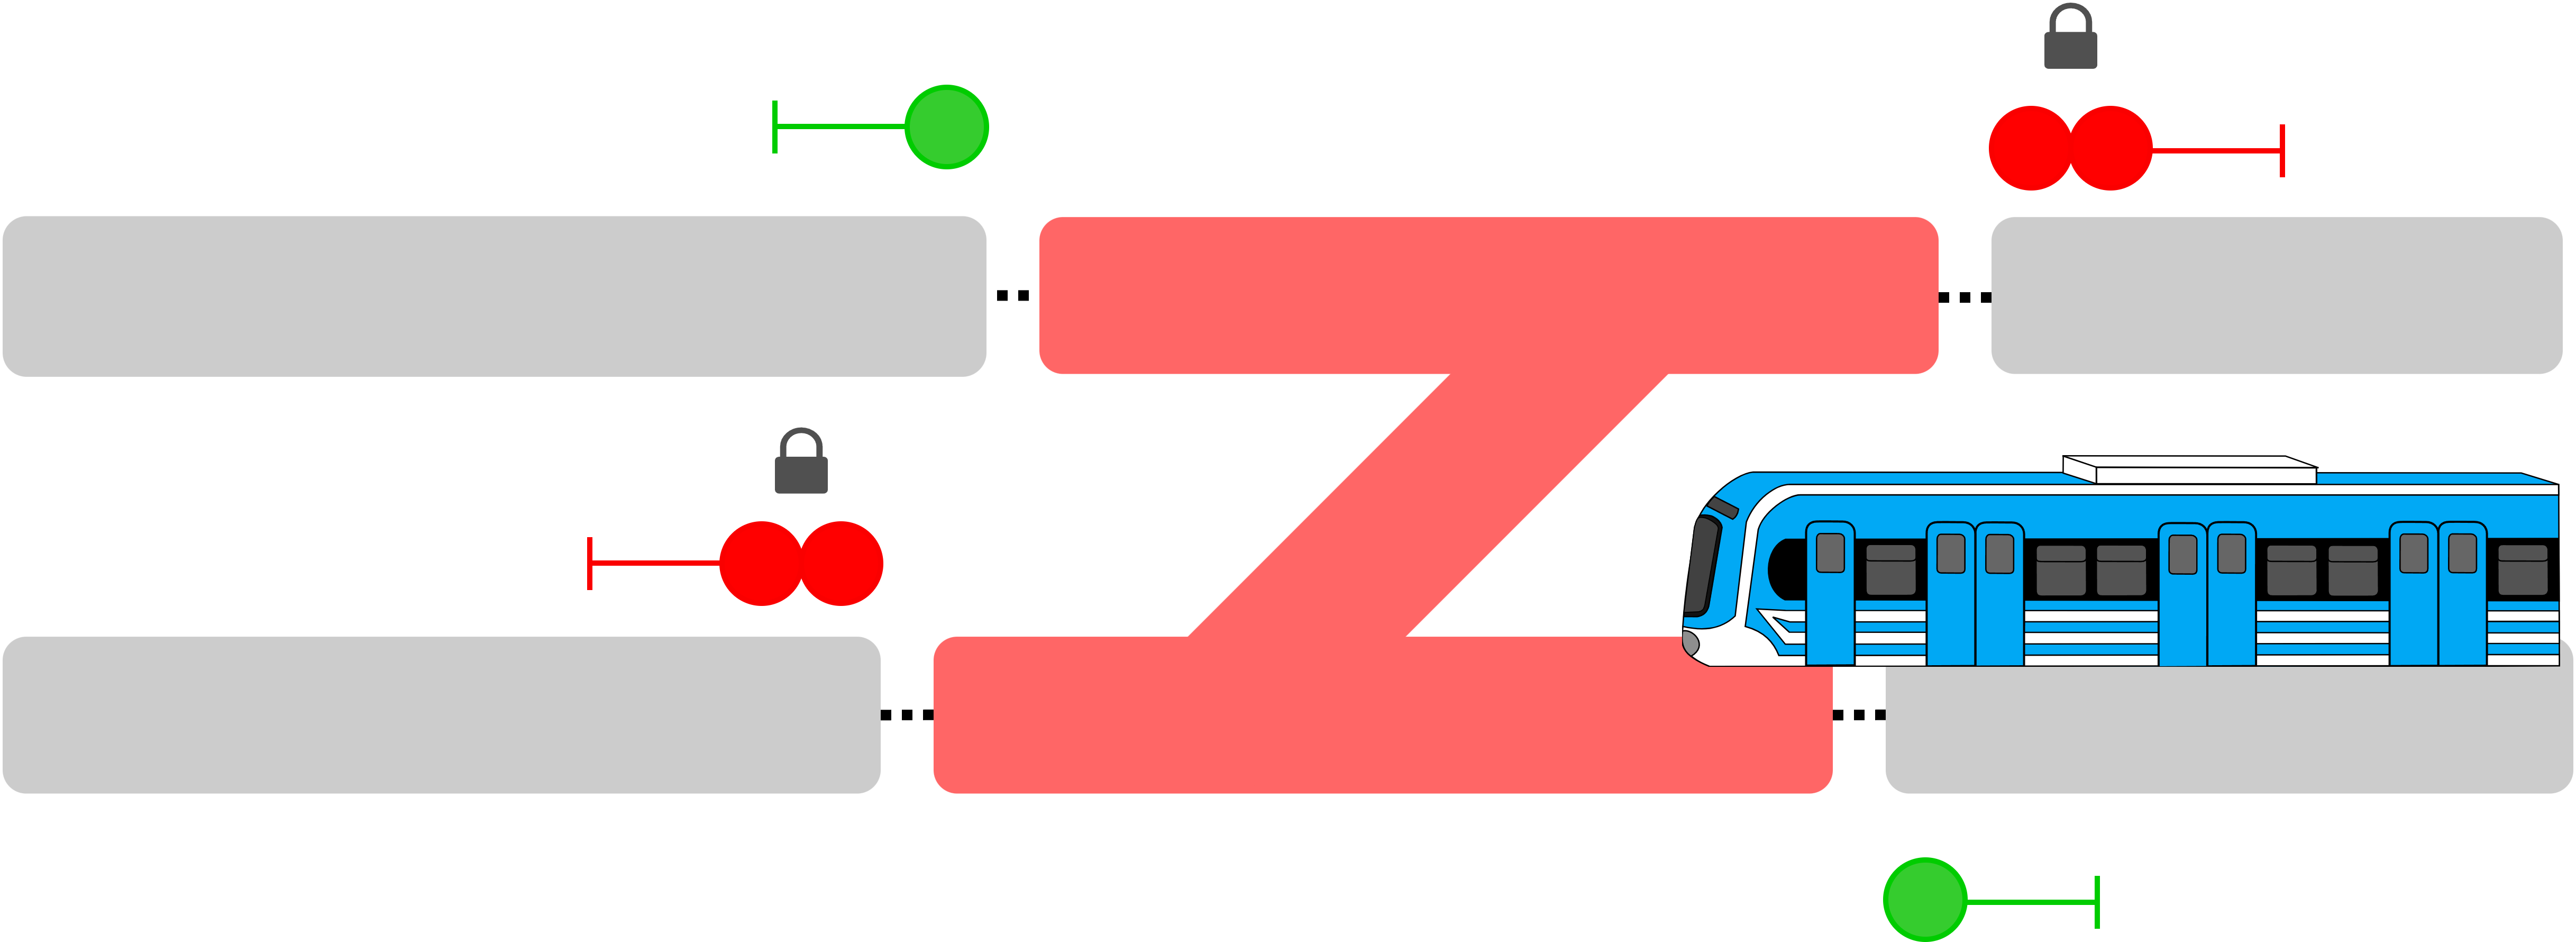
\includegraphics[width=0.7\textwidth]{Figuras/bloqueo_rutas}
        \centering\caption{Bloqueo de rutas conflictivas.}
        \label{fig:ACG_bloqueo}
    \end{figure}

	En el ejemplo de la Figura \ref{fig:ACG_bloqueo} se puede ver una formación que circula de derecha a izquierda por la vía inferior, al tener una señal verde que la habilita. El bloqueo de rutas conflictivas se manifiesta al forzar el aspecto rojo de las señales que habilitan dichas rutas, y al inhibir cualquier cambio de aspecto posible. Las rutas conflictivas pueden compartir todo el trayecto con la ruta principal, como la señal roja de la vía inferior; pero también pueden ser señales de rutas convergentes como la señal roja de la vía superior. De esta manera, se disminuyen las chances de colisiones frontales o laterales, respectivamente.
	
	